\section{Approach}
\label{sec:socvec}
We first discuss the intuition behind our model informally, then give the overall workflow of our approach, and finally present the details of the~\textit{\socvec}~framework. 

\subsection{Problem Statement and the Intuition}
Assuming the language $L_1$ is English and $L_2$ is Chinese,\footnote{Since the cross-cultural differences between eastern and western cultures are salient, 
this paper mainly considers English and Chinese as the target languages. 
Nevertheless, the techniques developed here are language independent and 
thus can be used for any two natural languages so long as 
we have a bilingual lexicon for the pair and a social-linguistic lexicon 
for one of the languages.} the problem we want to solve is, given 
an English term $W$ and a Chinese term $U$, compute a cross-lingual 
similarity score, $clsim(W, U)$, representing the cross-cultural 
similarity between $W$ and $U$. 

Although we can easily train English and Chinese word embeddings 
with the same dimensionality respectively, we cannot directly calculate 
the similarity between the word vectors of $W$ and $U$ since they 
are trained separately and thus the meaning of their dimensions 
are incompatible.
Consequently, we have to devise a reasonable way to calculate the 
similarity across heterogeneous vector spaces while retaining 
socio-linguistic information at the same time. 

A very intuitive solution to the problem is to translate $U$ to its English 
counterpart $U'$ through a bilingual lexicon and then simply consider 
the cosine similarity between $W$ and $U'$ by their word embeddings 
in the English word vector space.
However, this solution is infeasible under two situations: 
i) if $U$ is an OOV (Out of Vocabulary) term, e.g., a slang term, 
then there is no $U'$ in the bilingual lexicon; 
ii) if $W$ and $U$ refer to the same named entity, $U' = W$, 
then $clsim(W, U)$ is just the similarity between $W$ and itself, 
therefore we cannot capture any cross-lingual difference between 
$W$ and $U$, not to mention cross-cultural differences. 
Besides, this approach does not purposely preserve the 
cultural and social context of the terms. 
Therefore, this solution is not suitable for any of the two aforementioned 
tasks, which require the cross-cultural similarities between slang terms 
and differences between entity names.

To overcome the above problems, our intuition is thus 
to project English and Chinese word vectors to a common third space, 
known as \textit{\socvec} and this projection is supposed to carry 
\emph{socio-linguistic} context such as opinions, sentiments and cognition 
associated with the terms in respective languages. 
Such information will be encoded as values on each 
dimension of \textit{\socvec}.
%Considering the shortcomings of aforementioned transformation-based solutions, we propose to  
%construct a cross-lingual vector space with respect to sociolinguistic features, instead of transforming a space into another one.
%To construct a universal vector space for multilingual usage, we have to specify the meaning of each dimension for each language.
%Meanwhile, the meaning of the dimensions has to be related to opinion, sentiment, cognition and many other psychological processes to help capture the sociolinguistic information.
%Based on these two requirements, we argue that we should build a Bilingual Sociolinguistic Lexicon and extract word representation using the similarities to each translation pair in BSL as a medium.
%
\begin{figure}[th!]
	\centering
	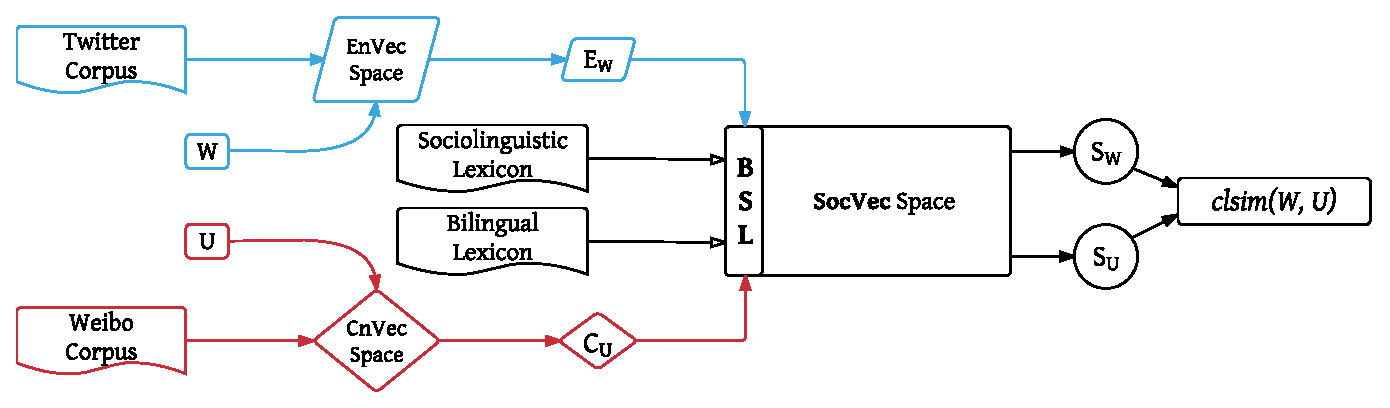
\epsfig{file=figures/overview.pdf, width=0.8\columnwidth}
	\caption{Workflow for computing the cross-cultural similarity between an English word \textit{W} and a Chinese word \textit{U}. $E_x$, $C_x$ and $S_x$ denote the word vectors of word $x$ (either $U$ or $W$) in \textit{EnVec} space, \textit{CnVec} space and \textit{SocVec} space respectively.  }
	\label{fig:overview}
\end{figure}

\subsection{Overall Workflow}
The \textit{\socvec}~model attacks the problem with the help of three low-cost external resources: 
i) English Twitter corpus and Chinese Weibo corpus; ii) a bilingual lexicon (\textit{BL}) between 
 English and Chinese common words;  
iii) English and Chinese socio-linguistic vocabularies 
(\textit{ESV} and \textit{CSV}).
For convenience, the words in these vocabularies are called
{\em social words}. Examples of social words in English include
\textit{fawn, inept, tremendous, gratitude,
terror, terrific, kiss, loving, traumatic}~\footnote{There are open-sourced
resources for these words as Section 3.1.4 describes.}
%\BL{maybe use another expression for the social words} 

\figref{fig:overview} shows the workflow of our framework to construct \textit{\socvec}~and compute $clsim(W,U)$. First, we train English and 
Chinese word embeddings (\textit{EnVec} and \textit{CnVec}) 
on the Twitter and Weibo corpora respectively. Then 
we build a bilingual socio-linguistic lexicon (\textit{BSL}) 
from the bilingual lexicon, CSV and ESV. 
The \textit{BSL} helps us 
map previously incompatible \textit{EnVec} and \textit{CnVec} 
into the common higher-dimensional \textit{\socvec~}space in which
two new vector representations, $S_W$ for $W$ and $S_U$ for $U$,
are now comparable to each other. 

\subsection{SocVec Modeling}
\label{sec:model}
In this section, we present the details of building the \textit{BSL} 
and constructing the \textit{\socvec} space.

\subsubsection{Building the BSL}
The process of building the \textit{BSL} is 
illustrated in~\figref{fig:BSL}. 
We first use the bilingual lexicon to translate each social word 
in the \textit{ESV} into Chinese words and then filter out any Chinese words 
that are not in the \textit{CSV}. After that, we have a set of 
Chinese social words translated from each English social word. 
We call this set of Chinese words the ``translation set''.
The final step is to generate a Chinese ``pseudo-word'' 
for each English social word.\footnote{A pseudo-word can be either 
an existing word that is the most representative word of the translation set 
or a fabricated word whose word vector is the combination of word vectors of
the translation set.}

\begin{figure}[th]
	\centering
	\epsfig{file=figures/BSL.pdf, width=0.9\columnwidth}
	\caption{Generating an entry in BSL for ``\textit{fawn}'' 
		and its pseudo-word ``\textit{fawn}*''.}
	\label{fig:BSL}
\end{figure}

For example, in \figref{fig:BSL}, the
English social word ``\textit{fawn}'' has three Chinese translations in the 
bilingual lexicon, but only two of them are social words. 
The pseudo-word generator takes the word vectors of the two words, namely
奉承(flatter) and 谄媚(toady), as input, and generates the pseudo-word 
vector of ``\textit{fawn}'', denoted as ``\textit{fawn*}''. 
%\footnote{The reason why we use the direction from English to Chinese  is that English socio-linguistic vocabularies tend to be more accessible and accurate than low-resource languages. The filter is optional for low-resource language which has no socio-linguistic lexicon, if we can afford the inaccuracy.}

Given an English social word $s$, we denote $\mathbf{C_i}$ as 
word vector of the $i^{th}$ word of the translation set of
size $N$. We design four types of pseudo-word generator as follows: 

\begin{align*}
	\intertext{\textbf{Max.}: Maximum of the values in each dimension, 
assuming $K$-dimensional word vectors.}
	Pseudo(\mathbf{C_1},...,\mathbf{C_N}) &= \begin{bmatrix}
	max(C_1^{(1)},...,C_N^{(1)}) \\
	\vdots   \\
	max(C_1^{(K)},...,C_N^{(K)})
	\end{bmatrix}^{\rm T} \\
	\intertext{\textbf{Avg.}: Average of the values in each dimension.}
	Pseudo(\mathbf{C_1},...,\mathbf{C_N})&=\frac{1}{N}\sum_i^N\mathbf{C_i} \
	\intertext{\textbf{W.~Avg.}: Weighted average value of each dimension 
with respect to the translation confidence (see~\secref{sec:blpre}).} 
	Pseudo(\mathbf{C_1},...,\mathbf{C_N})&=\frac{1}{N}\sum_i^Nw_i \mathbf{C_i} \
	\intertext{\textbf{Top}: Choose the most confident translation, $\mathbf{C_{top}}$.}
	Pseudo(\mathbf{C_1},...,\mathbf{C_N}) &= \mathbf{C_{top}} \
\end{align*}

At the end of this step, the BSL contains a set of English-Chinese word 
vector pairs, each representing an English social word and 
its Chinese pseudo-word.

\subsubsection{Constructing the \socvec~Space}
\label{sec:pg}
\textbf{Notation Definition.} 
We denote $\bf{E_x}$, $\bf{C_x}$ and $\bf{S_x}$ as the word vectors of 
word $x$ in \textit{EnVec}, \textit{CnVec} and \textit{\socvec} spaces
respectively.  Let $B_i$ be an English word and $B_i^*$ be
the corresponding Chinese pseudo-word in \textit{BSL} of size $L$. 

We can map an English word vector $\bf{E_W}$ into \textit{\socvec} by 
computing the cosine similarity between $\bf{E_W}$ and every English
word vector in \textit{BSL}, effectively constructing a new vector
$\bf{S_W}$ of size $L$. We can similarly map a Chinese word vector 
$\bf{C_U}$ into a new vector $\bf{S_U}$. 
Now $\bf{S_W}$ and $\bf{S_U}$ belong to the same vector space \textit{\socvec} 
and are comparable. 

For example, if $W$ is ``nagoya'' and $U$ is ``名古屋'', we compute the
cosine similarities between ``nagoya'' and ``fawn'', ``inept'', etc. in 
{\em EnVec} space, to form a vector of size $L$. This vector is known
as $\bf{S_{\text{nagoya}}}$. Similarly, we compute the cosine similarities
between ``名古屋'' and the Chinese pseudo-words of 
``fawn'', ``inept'', etc., and form a new vector $\bf{S_{\text{名古屋}}}$. 

Formally, $clsim(W,U)$ is computed as:
{\small
\begin{align*}
&clsim(W,U) := f(\mathbf{E_\text{W}},\mathbf{C_\text U}) \\ 
&=sim\left(
\begin{bmatrix}
    cos(\mathbf{E_\text W},\mathbf{E_{ B_1}})\\
    \vdots \\
    cos(\mathbf{E_\text W},\mathbf{E_{B_L}})
\end{bmatrix}^{\rm T},\begin{bmatrix}
    cos(\mathbf{C_\text U},\mathbf{C_{B_1^*}})\\
    \vdots \\
    cos(\mathbf{C_\text U},\mathbf{C_{B_L^*}})
\end{bmatrix}^{\rm T}\right)\\
&=sim(\mathbf{S_\text W},\mathbf{S_\text U}) 
\end{align*}}
where $cos$ denotes the cosine similarity, 
while $sim$ is a generic similarity function, for which a number of
metrics will be considered later in \secref{sec:eval}.
%
%to project $\mathbf{E_W}$ and $\mathbf{C_U}$ to $\mathbf{S_W}$ and $\mathbf{S_U}$ so that they can be comparable to each other.
%We define the function $f$ to compute cross-lingual similarity between $W$ and $U$ as follows.\footnote{Here $cos$ stands for cosine similarity, } This calculation process is also shown in ~\algref{alg:alg1}. \\
%
%\begin{algorithm}[th]
%	\small
%	\DontPrintSemicolon
%	\caption{Compute cross-lingual similarity between an English word 
%		\textit{W} and a Chinese word \textit{U} } 
%	\label{alg:alg1}
%	\KwIn{ \textit{EnVec}, \textit{CnVec}, $BSL$ with $L$ word pairs} 
%	\KwOut{the cross-lingual similarity $clsim(W,U)$} 
%	$E_W$ = word vector of $W$ in \textit{EnVec}\\
%	$C_U$ = word vector of $U$ in \textit{CnVec}\\
%	$S_W$ =  zero vector with $L$ dimension \\
%	$S_U$ =  zero vector with $L$ dimension \\
%	%	\Comment*[l]{Project $E_W$ into $S_W$}
%	\For{$1 \le i \le L$}{
%		$B_i$ =  $i^{th}$ English word in \textit{BSL} \\
%		$B_i^*$ = Chinese pseudo-word of $B_i$ \\
%		$S_W[i]$ = $cos(E_W,E_{B_i})$\\
%		$S_U[i]$ = $cos(C_U,C_{B_i^*})$\\
%	} 
%	\Return $clsim(W,U)$ = $sim(S_W,S_U)$\\
%\end{algorithm}
%\begin{figure}[th!]
%	\centering
%	\epsfig{file=figures/SocVec.pdf, width=0.6\columnwidth}
%	\caption{Using \textit{BSL} to project $E_W$ and $C_U$ to $S_W$ and $S_U$.}
%	\label{fig:swsu}
%\end{figure}

%\subsubsection{Parameters Description}
%\label{sec:pd}
%Here, we briefly summarize the main parameters of \textit{SocVec} model:
%\begin{itemize}
%\item Two trained monolingual word embeddings, \textit{EnVec} and \textit{CnVec};  
%\item A bilingual lexicon;
%\item Chinese and English socio-linguistic vocabularies; 
%\item Pseudo-word generator function; 
%\item Option of similarity function $sim$; 
%\end{itemize} 
%We conduct several experiments for testing the these parameters in~\secref{sec:mcdne}.
